\textbf{Ejemplo 5}\\

Dadas las alternativas A, B y C determinar la mejor alternativa usando el método de la TIRI
suponiendo que la TMAR= 25\%, compruebe el resultado usando el VPN. Las inversiones iniciales y el costo anual de operación (CAO) son: \\

\begin{center}
	
	\begin{tabular}{|c|c|c|c|}
		\hline
		\begin{tabular}[c]{@{}c@{}}\textbf{Proyecto}\end{tabular} & \begin{tabular}[c]{@{}c@{}}\textbf{A} \end{tabular} & \begin{tabular}[c]{@{}c@{}}\textbf{B} \end{tabular} & \begin{tabular}[c]{@{}c@{}}\textbf{C} \end{tabular} \\ \hline
		
		Costo                      &  COP  100.000                  &  COP  120.000                  &  COP  110.000                  \\ \hline
		
		CAO año 1                   &  COP  10.000                   &  COP  2.000                    &  COP  5.500                    \\ \hline
		
		CAO año 2                   &  COP  12.000                   &  COP  3.000                    &  COP  6.000                    \\ \hline
		
		CAO año 3                   &  COP  14.000                   &  COP  4.000                    &  COP  7.000                    \\ \hline
		
		CAO año 4                   &  COP  16.000                   &  COP  5.000                    &  COP  8.500                    \\ \hline
	\end{tabular}
	
\end{center}

\textbf{Solución.}\\
%La tabla ira centrada
\begin{center}
	\renewcommand{\arraystretch}{1.5}% Margenes de las celdas
	%Creación de la cuadricula de 3 columnas
\begin{longtable}[H]{|c|c|c|}
		%Creamos una linea horizontal
\hline
		%Definimos el color de la primera fila
\rowcolor[HTML]{FFB183}
%%%%% INICIO ASIGNACIÓN PERÍODO FOCAL %%%%%%%
  %%%%%%%%%% INICIO TITULO
  %Lo que se hace aquí es mezclar las 3 columnas en una sola
  \multicolumn{3}{|c|}{\cellcolor[HTML]{FFB183}\textbf{1. Asignación período focal}}   \\ \hline
  %%%%%%%%%% FIN TITULO
  %%%%% INICIO DECLARACIÓN DE VARIABLES %%%%%%%
  \multicolumn{3}{|c|}{$pf = O pmv$}   \\ \hline
  
%%%%%%%%%%% INICIO TITULO
\rowcolor[HTML]{FFB183}
\multicolumn{3}{|c|}{\cellcolor[HTML]{FFB183}\textbf{2. Declaración de variables}}    \\ \hline
%%%%%%%%%%% FIN TITULO
%%%%%%%%%%% INICIO MATEMÁTICAS

$ n = 5 pmv $                                     & \multicolumn{2}{c|}{$ VPN(A)=  COP  ? $} \\
$ \text{Inversión inicial} =  COP  20.000 $	& \multicolumn{2}{c|}{$ VPN(B)=  COP  ? $} \\
$ \text{Periodo 1 ingreso} =  COP  8.000 $	&	\multicolumn{2}{c|}{ $ VPN(C)=  COP  ? $ } \\
$ \text{Periodo 2 ingreso} =  COP  9.000 $	&	\multicolumn{2}{c|}{ $ $ } \\ 
$ \text{Periodo 3 ingreso} =  COP  10.000 $	&	\multicolumn{2}{c|}{ $  $ }
\\
$ \text{Periodo 4 ingreso} =  COP  11.000 $	&	\multicolumn{2}{c|}{ $ $ }
\\
\hline
%%%%%%%%%% FIN MATEMÁTICAS
		%%%%% INICIO FLUJO DE CAJA
\rowcolor[HTML]{FFB183}
\multicolumn{3}{|c|}{\cellcolor[HTML]{FFB183}\textbf{3. Diagrama de flujo de caja}} \\ \hline
		%Mezclamos 3 columnas y pondremos el dibujo
		%%%%%%%%%%%%% INSERCIÓN DE LA IMAGEN
		%Deberán descargar las imágenes respectivas del drive y pegarlas en la carpeta
		%n_capitulo/img/ejemplos/1/capitulo1ejemplo1.pdf  (el /1/ es el numero del ejemplo)
\multicolumn{3}{|c|}{ 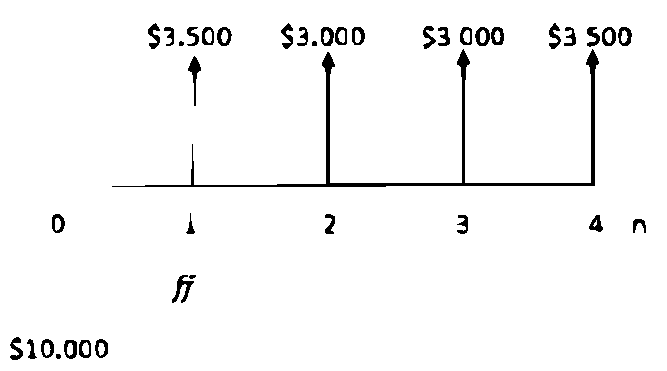
\includegraphics[scale=1, trim=-5 -5 -5 -5]{ejemplo6_2.png} }   
   \\\hline
		%%%%%%%%%%%%% FIN INSERCIÓN DE IMAGEN
		%%%%%FIN FLUJO DE CAJA
		
		
		
		%%%%% INICIO DECLARACIÓN FORMULAS
		%%%%%%%%%%% INICIO TITULO
\rowcolor[HTML]{FFB183}
\multicolumn{3}{|c|}{\cellcolor[HTML]{FFB183}\textbf{4. Declaración de fórmulas}}    \\ \hline
		%%%%%%%%%%% FIN TITULO
		%%%%%%%%%%% INICIO MATEMÁTICAS
\multicolumn{3}{|c|} {VPN =	$\sum F_{n}(1+i)^{-n}$   Valor presente neto.}   \\ 
\multicolumn{3}{|c|} {VPN =	$i=j/m$}   \\
\hline	
	
		%%%%%%%%%% FIN MATEMÁTICAS
		%%%%%% INICIO DESARROLLO MATEMÁTICO
\rowcolor[HTML]{FFB183}
		%%%%%%%%%%INICIO TITULO
\multicolumn{3}{|c|}{\cellcolor[HTML]{FFB183}\textbf{5. Desarrollo matemático}}       \\ \hline
		%%%%%%%%%% FIN TITULO
		%%%%%%%%%% INICIO MATEMÁTICAS
		\multicolumn{3}{|c|}{$ VPN(B-A): - COP  20.000 + COP   8.000(1+i)^{-1} +  COP  9.000(1 +i)^{-2}+  COP  10.000(1 +i)^{-3} + $}
		\\
		\multicolumn{3}{|c|}{$  COP  11.000(1+0)^{-4} =  COP  0 $}  
		\\
		\multicolumn{3}{|c|}{$ \text{Como la TIRI es mayor a la TMAR se concluye que el exceso } $}  
		\\
		\multicolumn{3}{|c|}{$ \text{de inversión ( COP  20.000) genera un interés del} $}  
		\\
		\multicolumn{3}{|c|}{$ \text{29.67\% pmv superior a la TMAR que es del 25\% pmv}$}  
		\\
		\multicolumn{3}{|c|}{$ \textbf{Observe que tenemos que tomar B-C para que la diferencia en 0 sea negativa,}$}  
		\\
		\multicolumn{3}{|c|}{$ \text{si lo tomamos invertido C-B la diferencia resulta positiva} $}  
		\\
		\multicolumn{3}{|c|}{ 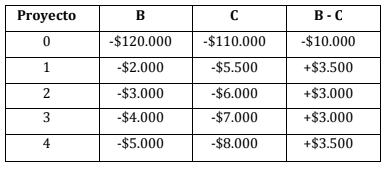
\includegraphics[scale=1, trim=-5 -5 -5 -5]{tabla_desarrollo_matematico_ejm6.png} }   
		\\
		\multicolumn{3}{|c|}{$ \text{Y su respectivo diagrama de flujo de caja:} $}  
		\\
		\multicolumn{3}{|c|}{ 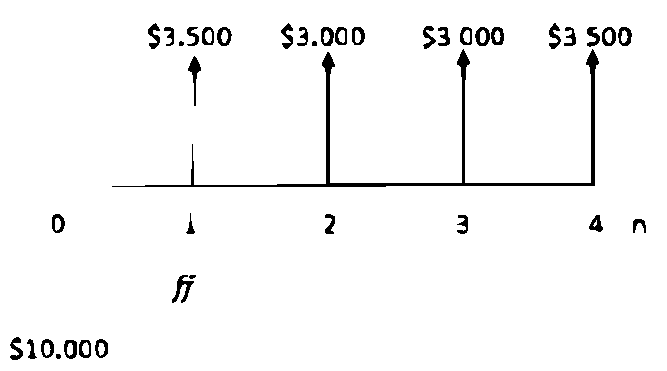
\includegraphics[scale=1, trim=-5 -5 -5 -5]{ejemplo6_2.pdf} }   
		\\
		\multicolumn{3}{|c|}{$ VPN(B-C)=:- COP  10.000 +  COP  3.500(1+i)^{-1} + COP  3.000(1+i)^{-2} + COP  3.000(1+i)^{-3} + $}
		\\
		\multicolumn{3}{|c|}{$ COP  3.500(1+i)^{-4} =  COP  0 $}   
		\\
		\multicolumn{3}{|c|}{$ \text{TIRI = 11.41\% pmv, lo cual nos indica que el excedente de inversión ( COP  10.000) genera un interés del} $}  
		\\
		\multicolumn{3}{|c|}{$\text{1.41\% pmv que es inferior a la TMAR, en consecuencia, el proyecto más costoso no es aconsejable por} $}  
		\\
		\multicolumn{3}{|c|}{$ \text{ lo tanto nos quedamos con el proyecto C.} $}  
		\\
		\multicolumn{3}{|c|}{$ \textbf{Se concluye así, que si B > A y C > B entonces C > B > A } $}  
		\\
		\multicolumn{3}{|c|}{$ \textbf{ por lo tanto la decisión final es invertir en el proyecto C.} $}  
		\\
		\multicolumn{3}{|c|}{$\text{Comprobación de la decisión usando el VPN usando la TMAR.}$}  
		\\ 
		\multicolumn{3}{|c|}{$VPN(B)= $}  
		\\
		\multicolumn{3}{|c|}{$ - COP  120.000 -  COP  2.000(1+0.025)^{-1} -  COP  3.000(1+0.25)^{-2} -  COP  4.000(1+0.25)^{-3} - $}
		\\
		\multicolumn{3}{|c|}{$  COP  5.000(1+0.25)^{-4}$}  
		\\
		\multicolumn{3}{|c|}{$ VPN(B)= - COP  127616 $}
		\\
		\multicolumn{3}{|c|}{$ VPN(C)=  $}  
		\\
		\multicolumn{3}{|c|}{$ - COP  110.000 -  COP  5.500(1+0.025)^{-1} - COP  6.000(1+0.25)^{-2}-  COP  7.000(1+0.25)^{-3}-0 $}
		\\
		\multicolumn{3}{|c|}{$  COP  8.500(1+0.25)^{-4} $}  
		\\
		\multicolumn{3}{|c|}{$ VPN(C)=-  COP  125.306 $}  
		\\
	    \hline
				
		%%%%%%%%%% FIN MATEMÁTICAS
		%%%%%% FIN DESARROLLO MATEMÁTICO
		%%%%%% INICIO RESPUESTA
\rowcolor[HTML]{FFB183}
		%%%%%%%%%%INICIO TITULO
\multicolumn{3}{|c|}{\cellcolor[HTML]{FFB183}\textbf{6. Respuesta}}   \\ \hline
		%%%%%%%%%% FIN TITULO
		%%%%%%%%%% INICIO RESPUESTA MATEMÁTICA
		
\multicolumn{3}{|c|}{ \text{El VPN mayor es el correspondiente al proyecto C, por tanto, debe}}
\\
\multicolumn{3}{|c|}{\text{escogerse este proyecto. La decisión es coincidente con la que } }
\\
\multicolumn{3}{|c|}{ \text{indica la TIRI.}}
\\
\hline

		
		%%%%%%%%%% FIN MATEMÁTICAS
		%%%%%% FIN RESPUESTA
	\end{longtable}
	%Se crean dos lineas en blanco para que no quede el siguiente texto tan pegado
	%\newline \newline %USARLO SI CREES QUE ES NECESARIO
\end{center}
%%%%%%%%%%%%%%%%%%%%%%%%%%FIN EJERCICIO 1 %%%%%%%%%%%%%%%%%%%%%%%%%%%


\textbf{}\\
